\section{Metodología de Seguimiento}

Para llevar un control detallado del desarrollo del proyecto, se ha utilizado un documento en formato Excel donde se han registrado diariamente las tareas realizadas. Cada entrada incluye los siguientes campos:

\begin{itemize}\setlength{\itemsep}{0pt}
    \item \textbf{Fecha}: Fecha en la que se ha realizado la tarea.
    \item \textbf{Sección}: Categoría de la tarea (documentación, diseño, análisis...).
    \item \textbf{Tarea}: Breve descripción de la actividad llevada a cabo.
    \item \textbf{Dedicación}: Cantidad de horas empleadas dirante ese día.
    \item \textbf{Descripción}: Información más detallada sobre la tarea, incluyendo detalles relevantes que puedan ser útiles para futuras referencias.
    \item \textbf{Incidencias}: Problemas o dificultades encontradas.
    \item \textbf{Soluciones}: Posibles soluciones planteadas.
\end{itemize}

Gracias a este sistema de seguimiento, se ha podido llevar un control preciso del tiempo dedicado al proyecto y de la distribución de esfuerzos en las distintas fases. Además, con un total de 94 registros en este documento, se han podido documentar incidencias, decisiones y cambios en el alcance del proyecto, lo que ha facilitado la trazabilidad de su evolución.


\section{Materialización de Riesgos}

A lo largo del desarrollo del proyecto, se han materializado algunos de los riesgos identificados en la planificación inicial. Aunque estos riesgos afectaron de diversas formas al desarrollo, la planificación anticipada y las estrategias de mitigación permitieron minimizar sus efectos, asegurando que el TFG pudiera completarse dentro de los plazos establecidos. A continuación, se detallan los principales riesgos materializados:

\newpage

\subsection*{R01: Limitaciones con respecto a los datos disponibles de la API}

Uno de los primeros riesgos que afectaron al desarrollo del proyecto fue la disponibilidad limitada de ciertos datos en la API de \textit{Spotify}. Durante la fase inicial de validación, se comprobó que algunas de las estadísticas planteadas en la planificación no podrían implementarse debido a restricciones sobre los datos. En particular, el historial de canciones escuchadas por el usuario estaba limitado a las últimas 50 reproducciones, lo que impedía generar métricas a largo plazo.

Ante esta situación, fue necesario descartar dos de las estadísticas originales y replantear nuevas alternativas que se ajustaran a la información accesible. Este ajuste se llevó a cabo durante la primera iteración del desarrollo, en la cual se realizó un prototipado rápido para evaluar la viabilidad de distintas soluciones.

\subsection*{R02: Cambios en la política de acceso a la API}

Uno de los riesgos con mayor impacto en el proyecto fue la deprecación de varios endpoints de la API de \textit{Spotify}, anunciada el 27 de noviembre de 2024 en su blog oficial. Esta modificación inesperada obligó a replantear algunas de las estadísticas previstas, ya que varias funcionalidades dejaron de estar disponibles. En particular, la eliminación de los endpoints de \textit{Audio Features} y \textit{30-second preview URLs}, que se tomaron como base para el desarrollo.

Afortunadamente, el anuncio se realizó cuando el desarrollo se encontraba aún en una fase temprana de implementación, lo que permitió adaptar el proyecto sin afectar gravemente al progreso general. La principal acción tomada fue el rediseño de las estadísticas utilizando los datos aún accesibles en la API. Como resultado, se eliminó una de las métricas iniciales y se diseñó una nueva, siendo esta \textit{Índice de Interferencia}, presente en la implementación final.

\subsection*{R04: Incompatibilidad de versiones de las tecnologías utilizadas}

Aunque este riesgo no tuvo un impacto crítico en la funcionalidad de la aplicación, sí generó desviaciones en la planificación, especialmente en las fases de pruebas y despliegue. Se encontraron problemas de compatibilidad con ciertas dependencias a la hora de implementar las pruebas con Jest.

El mayor desafío se presentó al implementar la ejecución automática de pruebas en \textit{GitHub Actions}, donde fue necesario realizar múltiples pruebas con distintas configuraciones hasta encontrar una que funcionara correctamente. Si bien este problema supuso un retraso en el apartado de testing, no comprometió el desarrollo del resto de funcionalidades y se logró estabilizar la integración continua tras varios ajustes.

\subsection*{R06: Dificultad para compaginar el proyecto con las obligaciones académicas}

Desde el inicio del proyecto se identificó el riesgo de que la carga académica afectara al progreso del TFG, especialmente debido a la necesidad de aprobar una asignatura en diciembre para poder presentar el trabajo en febrero. Como medida preventiva, se realizó un ajuste en la distribución del tiempo de trabajo durante ese periodo, priorizando el estudio en las dos semanas previas al examen, que tuvo lugar el 16 de diciembre.

Si bien esto supuso una reducción temporal en la dedicación al TFG, la estrategia de mitigación permitió redistribuir el esfuerzo en semanas posteriores sin causar un impacto significativo en el desarrollo global del proyecto. Gracias a esta previsión, no fue necesario realizar modificaciones drásticas en los plazos generales y se pudo retomar el ritmo normal de trabajo tras el periodo de exámenes.

\section{Desviaciones en el Alcance}

A lo largo del desarrollo del proyecto, el alcance general definido en la planificación inicial se ha mantenido sin alteraciones significativas. Las funcionalidades principales, tales como la autenticación con \textit{Spotify}, el panel de información del usuario, los gráficos interactivos y la interfaz responsiva, han sido implementadas según lo previsto. Del mismo modo, las exclusiones establecidas o las limitaciones identificadas no han sufrido modificaciones.

No obstante, a nivel de funcionalidad específica, se han producido ciertos ajustes derivados de los riesgos materializados ya mencionados, que ocurrieron en los siguientes dos puntos:

\begin{itemize}
    \item \textbf{Incremento I: Prototipado Rápido}:  El riesgo \textbf{R01} se dió durante el análisis de viabilidad, se determinó que algunas estadísticas no podían implementarse debido a la falta de acceso a datos históricos de escucha.
    \item \textbf{Incremento II: Producto Mínimo Viable (PMV)}: Tras el anuncio de \textit{Spotify} sobre la deprecación de varios endpoints de su API, plevisto como el riesgo \textbf{R02}.
\end{itemize}

Como resultado de estas modificaciones, de las seis estadísticas avanzadas inicialmente previstas, cuatro han llegado a la versión final del proyecto. En la siguiente figura \ref{fig:estadisticas_cambio} se presenta el resumen de estos cambios, indicando cuáles fueron descartadas, en qué fase se produjo la decisión y los motivos que llevaron a su eliminación o sustitución.

\begin{figure}[H]
    \centering
    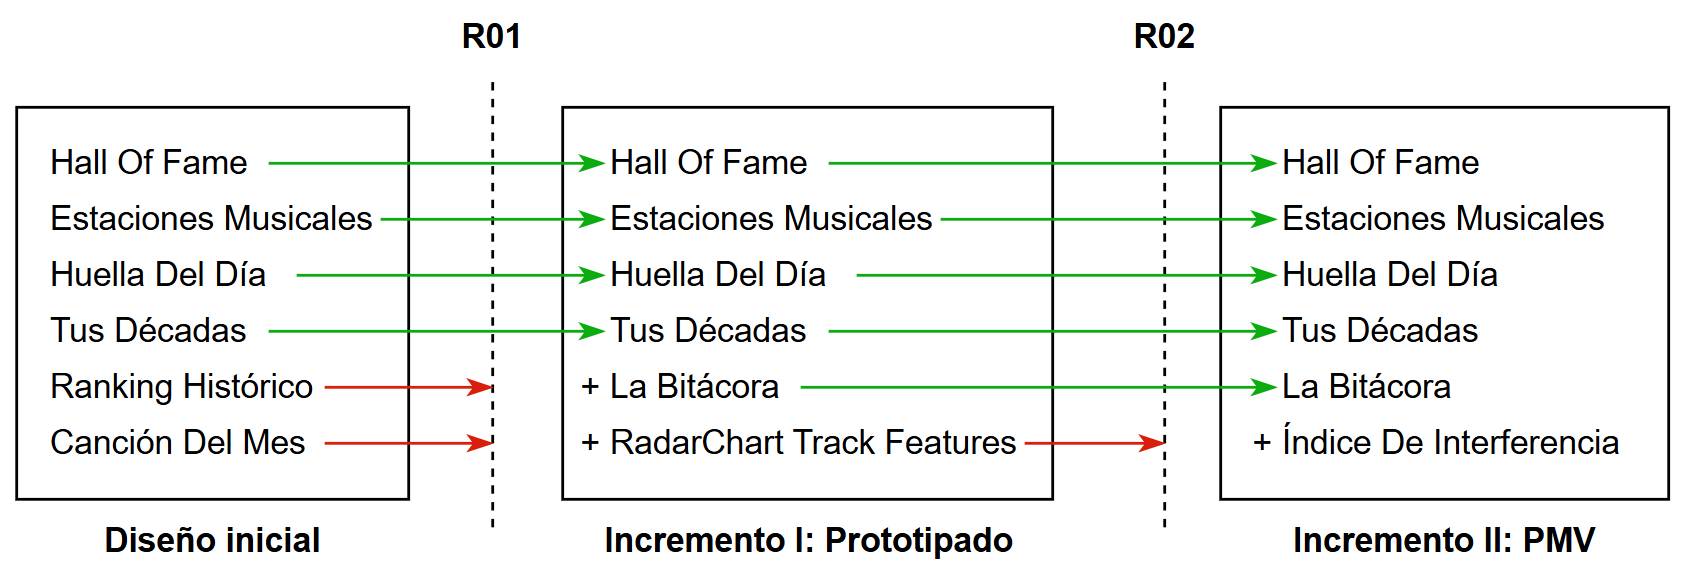
\includegraphics[width=0.9\textwidth]{figures/syc/estadisticas_cambio.png}
    \vspace{0.5cm}
    \caption{Resumen de cambios en la selección de estadísticas avanzadas.}
    \label{fig:estadisticas_cambio}
\end{figure}

\newpage

\section{Desviaciones Temporales}

Para evaluar la ejecución del proyecto respecto a la planificación inicial, se ha realizado un seguimiento continuo de los tiempos de dedicación y cumplimiento de tareas. Esto ha permitido ajustar plazos cuando ha sido necesario y asegurar que el desarrollo del proyecto se mantuviera dentro de unos márgenes aceptables.

\textbf{Estrategias de gestión de la planificación:}

\begin{itemize}
    \item \textbf{Monitoreo periódico}: Se han registrado las horas dedicadas a cada tarea y se ha comparado con lo planificado.
    \item \textbf{Ajustes sobre la marcha}: En tareas críticas que tomaron más tiempo del esperado, se reorganizaron las actividades para evitar acumulación de retrasos.
    \item \textbf{Priorización de tareas}: Algunas funcionalidades se postergaron para evitar riesgos en la entrega del proyecto final.
\end{itemize}

Gracias a estas estrategias, se ha minimizado el impacto de los imprevistos en la planificación global del TFG.

\section{Revisión de Objetivos}

\section{Entregables Generados}

El desarrollo del proyecto ha dado lugar a una serie de entregables clave que documentan su progreso y resultados:

\begin{itemize}
    \item Código fuente de la aplicación.
    \item Documentación técnica sobre la arquitectura y la implementación.
    \item Memoria del TFG con todos los análisis y resultados obtenidos.
    \item Tablas de seguimiento con la dedicación real a cada tarea.
    \item Informes de pruebas y validación de la aplicación.
\end{itemize}

Estos entregables han sido fundamentales para garantizar la trazabilidad y calidad del proyecto.


